\documentclass[12pt,a4paper]{article}
\usepackage[utf8]{inputenc}
\usepackage[T1]{fontenc}


\renewcommand{\baselinestretch}{0.2}

\setlength{\hoffset}{-18pt}         
\setlength{\oddsidemargin}{0pt} % Marge gauche sur pages impaires
\setlength{\evensidemargin}{0pt} % Marge gauche sur pages paires
\setlength{\marginparwidth}{54pt} % Largeur de note dans la marge
\setlength{\textwidth}{481pt} % Largeur de la zone de texte (17cm)
\setlength{\voffset}{-18pt} % Bon pour DOS
\setlength{\marginparsep}{7pt} % Séparation de la marge
\setlength{\topmargin}{0pt} % Pas de marge en haut
\setlength{\headheight}{13pt} % Haut de page
\setlength{\headsep}{4pt} % Entre le haut de page et le texte
\setlength{\footskip}{27pt} % Bas de page + séparation
\setlength{\textheight}{720pt} % Hauteur de la zone de texte (25cm)
\setlength{\parindent}{0pt}

\usepackage{natbib}
\usepackage{graphicx}
\usepackage{array}
\usepackage{tabularx}
\usepackage{booktabs}
\usepackage[table]{xcolor}
\usepackage{amssymb}
\usepackage{amsmath} % Required for the align* environment
\usepackage{float}
\usepackage{pgfplots} 
\usepackage{algorithm}
\usepackage{mathrsfs}
\definecolor{tableheader}{RGB}{240, 243, 246}
\definecolor{rowstripe}{RGB}{248, 249, 250}

\usepackage{algpseudocode} % test comment
\usepackage[hidelinks]{hyperref}
\pgfplotsset{compat=1.18}


\begin{document}
\author{Yunshan Luo}
\title{ME2322 --- Industrial Transformation}
\maketitle
\newpage

\section{Course overview}
\textbf{Examination:}
\begin{itemize}
    \item Oral exam
    \item Written group assignment
\end{itemize}


\textbf{Intended learning outcomes:
}\begin{enumerate}
    \item Describe, explain use concepts, models and theories to analyze industrial dynamics and technological innvation applied to industrial development in Sweden
    \item Analyze the two-way relationship between societal challenges and industrial dynamics: challenges shape innovation and innovation shapes how society responds to challenges
\end{enumerate}

\textbf{Societal challenges:}
\begin{enumerate}
    \item AI-driven transformation and sustainable transitions 
    \item Guest lecture industries (food, energy, gaming, health)
    \item Focus on supply and demand side of technological innovation
\end{enumerate}

Key buzzwords:
\begin{itemize}
    \item \textbf{Industrial dynamics:} The study of how industries change over time: entry and exit of firms, growth and decline, the evolution of market structure. Dominant designs and GPTs explain why these dynamics happen
    \item \textbf{Technological innovation:} New or significantl improved products, processes, or services: \textbf{innovation is not an invention}, an innovation only becomes an innovation when it reaches the market and is adopted
    \item \textbf{Societal challenge:} A large, long-term, systemic problem that markets alone do not automatically solve (e.g. climate change, AI-driven transformation). Focus on AI-driven transformation and sustainable transitions.
    \item \textbf{Dominant design:} A product architecture that wins the allegiance of the market and becomes the industry standard
    \item \textbf{General purpose technology (GPT):} A technology that is pervasive, keeps improving and spawns complementary innovations across sectors
    \item \textbf{Technological innovation system (TIS):} The network of actors, institutions, and interactions that develops and diffuses a specific technology.
    \item \textbf{Multi-level perspective (MLP):} Explains transitions as interactions among three levels: niche innovations, the incumbent socio-technical regime and external landscape
    \item \textbf{Diffusion of innovations:} How new technologies spread through a population over time, and who adopts early vs late (adopters, change agents)
    \item \textbf{Critical perspective:} Questioning hidden assumptions in transition/innovation research e.g. who benefits, who is excluded and whether sustainability claims are real
\end{itemize}

\section{Lecture 1: Industrial dynamics, dominant design, GPTs}
\begin{itemize}
    \item Why does a industry of competing designs converge into one? 
    \item How does a technology become a GPT? Why hasn't AI become a GPT yet?
\end{itemize}

\subsection{Dominant design emergence}
\begin{enumerate}
    \item Industries begin in a \textbf{fluid phase} with many competing designs
    \item A \textbf{dominant design} emerges which wins the allegiance of the marketplace
    \item Product innovation slows down, process innovation accelerates
    \item The number of firms collapses in an \textbf{exit wave/shakeout}
\end{enumerate}

\textbf{Example (qwerty keyboard):}
\begin{itemize}
    \item Designed in 1873 which became the standard to avoid jamming of mechanical typewriters
    \item The design has remained largely unchanged since then
    \item Still used today in computers despite despite being suboptimal since jamming is no longer an issue
\end{itemize}

\textbf{Three phases of emergence:}
\begin{enumerate}
    \item \textbf{Fluid phase:} Rapid product innovation, competition is about novelty, many competing designs.
    \item \textbf{Transitional phase:} Emergence of a dominant design, markets begin to converge on one architecture.
    \item \textbf{Specific phase:} Dominant design has emerged, process innovation i.e. costs, quality, scale becomes the competition.
\end{enumerate}

\textbf{Key buzzwords:}
\begin{itemize}
    \item \textbf{Product innovation:} New designs, features, achritectures, etc. Focus on novelty and performance.
    \item \textbf{Process innovation:} New ways of producing existing products. Focus on cost, quality, and scale.
    \item \textbf{Exit wave/shakeout:} Decline in number of firms after dominant design emerges. Competition shfits to scale and cost.
    \item \textbf{Assembled/non-assembled product:} 
    \begin{itemize}
        \item \textbf{Assembled product:} Products that are put together from various components, such as cars, smartphones, etc. Emergence of a dominant design is is the landmark event
        \item \textbf{Non-assembled product:} Products that are components such as steel, chemicals, etc. Emergence of dominant process matter more than dominant design.
    \end{itemize}
    \item \textbf{Dominant process:} A production process that becomes the industry standard. Important for non-assembled products. Example: Bessemer process for steel production.
    \item \textbf{Enabling technology:} A process technology that incorporates needed elements that causes the industry shift from process innovation to process improvement. Example: float glass process for glass production.
    \item \textbf{Collateral assets:} Complementary assets that the firm already owns such as: brand, distribution channels, service networks, customer switching costs. Owning them helps push its design to dominance. Example 
    \begin{itemize}
        \item Apple's iPhone: brand, app store, etc.
        \item IBM's PC: brand, distribution channels, service networks, etc.
    \end{itemize}
    \item \textbf{Strategic maneuvering:} Firms decides which design wins example.
    \begin{itemize}
        \item VHS beat Betamax despite being technically inferior because JVC built alliances ("humble" strategy) while sony kept betamax proprietary.
    \end{itemize}
    \item \textbf{Lead users/producer-user communication:} Users who are at the forefront of innovation and can provide valuable feedback to producers.
    \item \textbf{Creative destruction:} A successful innovation creates a temporary monopoly with high margins, which attracts imitators which erodes the monopoly.
    \item \textbf{Technological trajectory/design hierarchy:} Once a technical concept is chosen later design decisions are constrained along a path. QWERTY keyboard locked all keyboard evolution onto one trajectory
    \item \textbf{Lock-in with complementary assets:} QWERTY persisted because users and firms had invested in typing skills as complementary assets. Switching to a better design would require re-learning and re-investing in complementary assets.
    \item \textbf{Enabling technology:} A process technology that incorporates needed elements that causes the industry shift from process innovation to process improvement. Example: float glass process for glass production.
\end{itemize}    

\textbf{Mapping buzzword to theory:}
\begin{enumerate}
    \item Fluid stage: Young assembled product has no firm lock. No mastered manufacturing processes, customers haven't formed an idea of the ideal product. Capital and technical barriers are low, entry is easy.
    \item What are the consequences of dominant design?
    \begin{itemize}
        \item \textbf{Performance requirements becomes implicit:} Windshield wipers ona car, shifting for upper and lowercase are expected by users. Firms that don't meet these requirements are excluded from the market.
        \item \textbf{Enforcing standardization:} Competition shifts from design novelty to cost, scale, and product performance.
        \item \textbf{Redirects and slows innovation:} For example for the QWERTY keyboard redesign is off-limits.
    \end{itemize}
    \item Dominant design is not predetermined rather the result of interplay between technology and market via four forces and inertia:
    \begin{itemize}
        \item \textbf{Collateral assets:} IBM's first PC had following collateral assets: brand value, expected service and parts and the software ecosystem.
        \item \textbf{Industry regulation and government:} FCC's approval of RCA's television broadcasting standard made RCA's design dominant.
        \item \textbf{Strategic maneuvering:} JVC's VHS beat Sony's Betamax because JVC built alliances with other firms while Sony kept Betamax proprietary.
        \item \textbf{Communication between producers and uesrs:} Staying close to customers shows firms which features truly matter.
        \item \textbf{Inertia and complementary assets:} QWERTY's persistence reflects the inertia of established practices i.e. typing skills. 
    \end{itemize}
    \item \textbf{Life-cycle signature:} Entry $\rightarrow$ peak $\rightarrow$ exit. The number of firms rises fast during the fluid stage peaks during the transitional stage and falls during the specific stage. 
    \item \textbf{Assembled vs non-assembled product:} For non-asssembled products experimentaiton is in the process and the emergence of a dominant process not product. A process enabling technology shifts the industry from process innovation to process improvement. 
\end{enumerate}

% Discuss the questions with someone
\newpage
Real industry cases:
\begin{figure}[H]
    \centering
    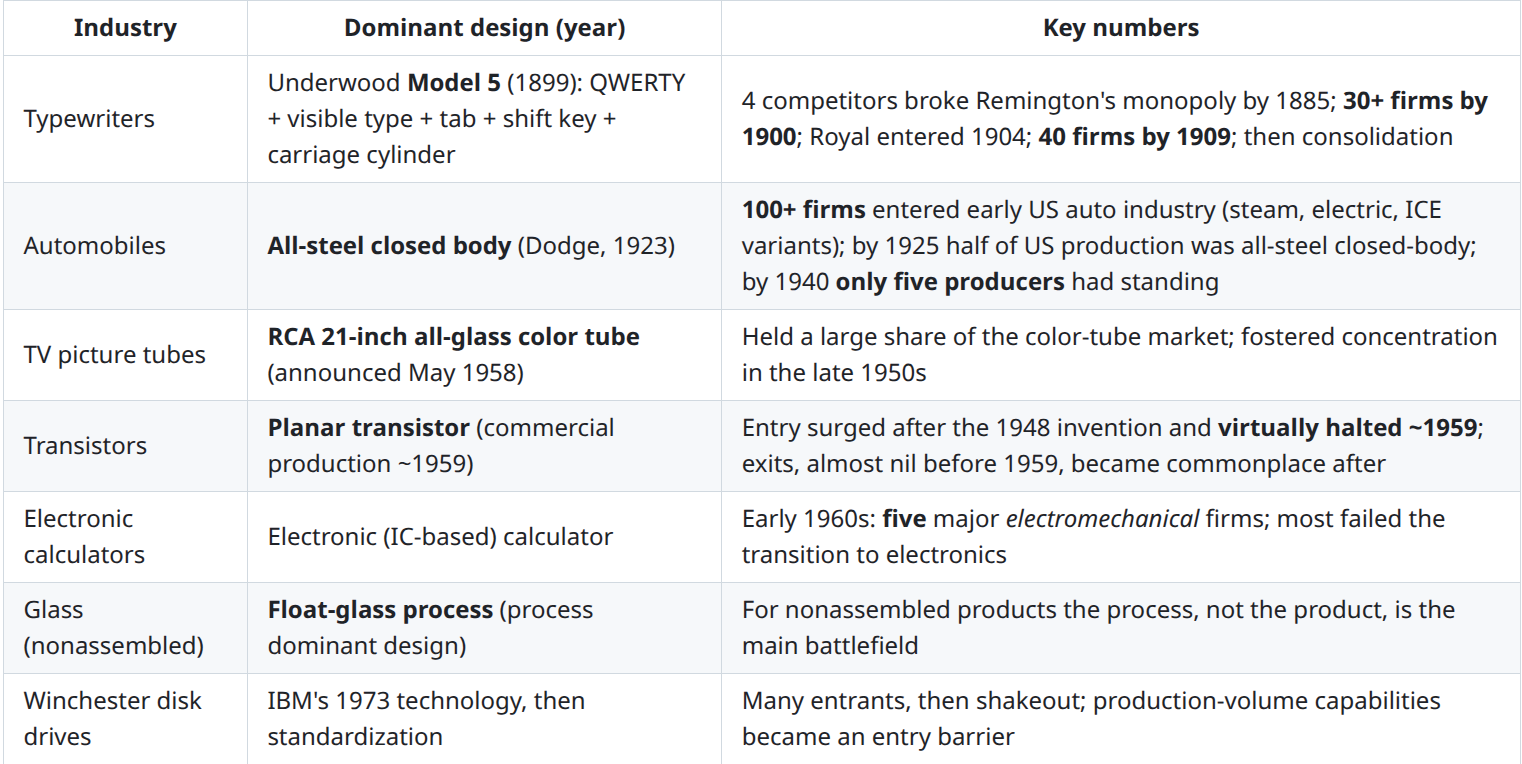
\includegraphics[width=1.1 \textwidth]{image1.png} 
\end{figure}

\subsection{What innovation paths for AI to become GPT}
General purpose technologies GPTs are for example electricity, steam engine and the internet. AI could become a GPT if it had an \textbf{GPT loop} --- positive feed back between improvements and application-sector coinvention.

\textbf{Key buzzwords:}


















\end{document}